\documentclass[class=report, crop=false, 12pt,a4paper]{standalone}
\usepackage{enumitem}
\usepackage{tikz}
\usetikzlibrary{shapes.geometric, arrows}
\usepackage{float}
\usepackage{graphicx}
\usepackage{multicol}
\usepackage{tabularx}
\renewcommand{\arraystretch}{1.5}
\usepackage{siunitx}
\usepackage{mathtools}
\usepackage{amsmath}
\usepackage{amssymb}
\usepackage{commath}
\usepackage[normalem]{ulem}
\usepackage[a4paper,width=150mm,top=25mm,bottom=25mm]{geometry}
\begin{document}
\subsection*{Stages in a measurement system}
\begin{figure}[H]
  \centering
  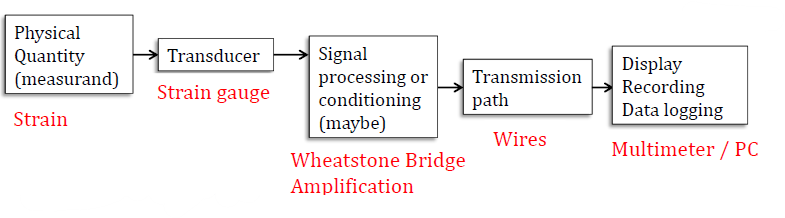
\includegraphics[width = 0.8 \textwidth]{../img/diagram38.png}
\end{figure}
\section{Amplifiers}
\begin{figure}[H]
  \centering
  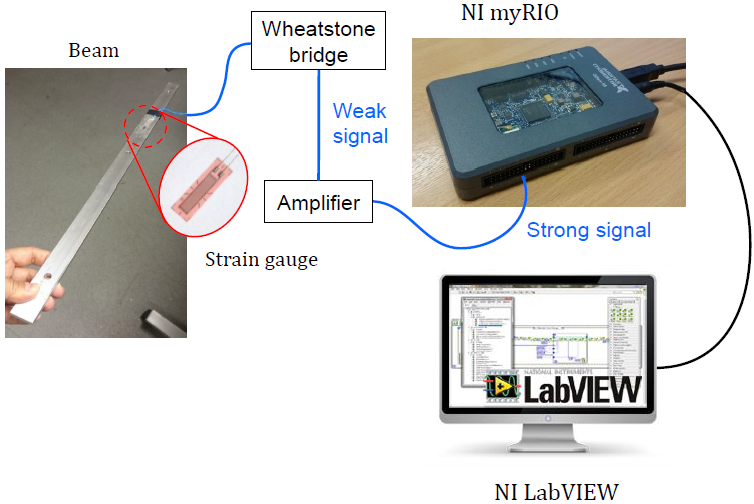
\includegraphics[width = 0.7\textwidth]{../img/diagram39.png}
\end{figure}
The voltage output from a transducer tends to be weak and this needs to be amplified. Operational amplifiers are normally around 1\si{\centi\meter} in size.
\begin{figure}[H]
  \centering
  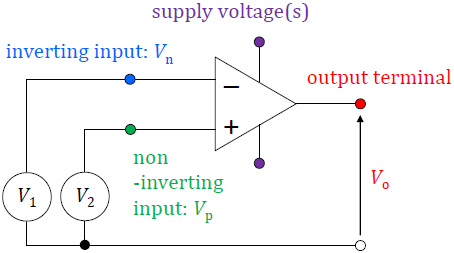
\includegraphics[width = 0.7\textwidth]{../img/diagram40.png}
\end{figure}
\begin{equation}
  V_0 = A_v (V_p - V_n) = A_v (V_2 - V_1)
\end{equation}
Where $A_v$ is the gain and $(V_p - V_n)$ can be from a Wheatstone bridge. Operational amplifiers are quite an old technology (since WW2) and are still used because they are cheap and convenient.
\begin{figure}[H]
  \centering
  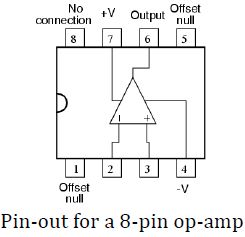
\includegraphics[width = 0.5\textwidth]{../img/diagram41.png}
\end{figure}
\begin{figure}[H]
  \centering
  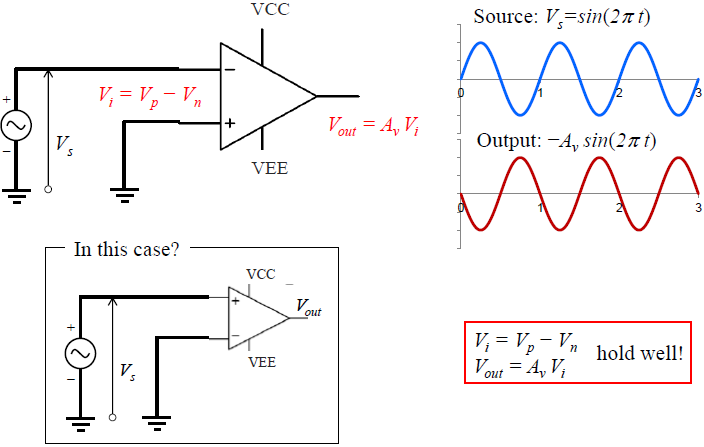
\includegraphics[width = 0.7\textwidth]{../img/diagram42.png}
\end{figure}
\subsection{Equivalent op-amp circuit and conditions of an ideal op-amp}
\begin{figure}[H]
  \centering
  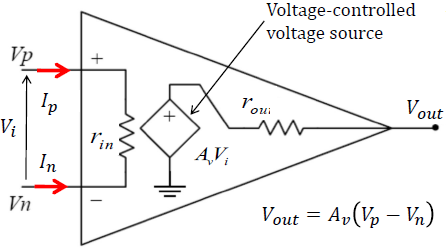
\includegraphics[width = 0.7\textwidth]{../img/diagram43.png}
\end{figure}
Terminology:
\begin{itemize}
  \item Differential input voltage: $V_i = V_p - V_n$
  \item Input resistance: $r_{in}$
  \item Output resistance: $r_{out}$
  \item Open-circuit output voltage: $V_{out}$
  \item Differential voltage gain: $A_v$
\end{itemize}
\begin{center}
  \begin{tabular}{ |c|c| } 
    \hline
    \textbf{Conditions of an ideal op-amp} & \textbf{In reality} \\
    \hline
    \hline
    No current into input terminals: $I_p = I_n = 0$ & \\
    \hline
    Infinite input resistance: $r_{in} \rightarrow \infty$ & $r_{in} > 200 \si{\kilo \ohm}$\\
    \hline
    Zero Output resistance $r_{out} = 0$ & $r_{out} < 1 \si{\kilo\ohm}$\\
    \hline
    Infinite differential (or open-loop) gain $A_v \rightarrow \infty$ & $A_v > 100,000$\\
    \hline
    Zero common-mode voltage gain $A_{cm} = 0$ & $A_v$ also frequency dependant\\
    \hline
  \end{tabular}
\end{center}
\subsection{Non-zero voltage with zero current?}
\begin{figure}[H]
  \centering
  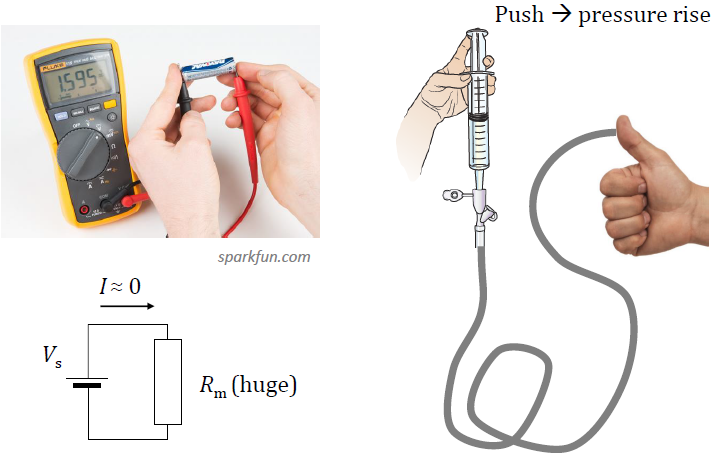
\includegraphics[width = 0.7\textwidth]{../img/diagram44.png}
\end{figure}
A question that is often asked is if the current is zero, how can we still have a voltage? When you connect a battery to a meter, where the meter resistance is normally huge. We can still measure the voltage. This is due to Ohm's law $I = \frac{V}{R_m}$. A good analogy to make is a plunger system, where the other end is covered. When you push down, increasing the pressure, this can still be felt on the tip of the thumb, despite there being no flow. In the same way, we can still 'feel' the voltage with 'no' current flow.
\subsection{Saturation}
In a practical scenario, we want to strengthen the weak signal from the sensor. Let us connect an input to the non-inverting terminal and the inverting input to the ground.
\begin{figure}[H]
  \centering
  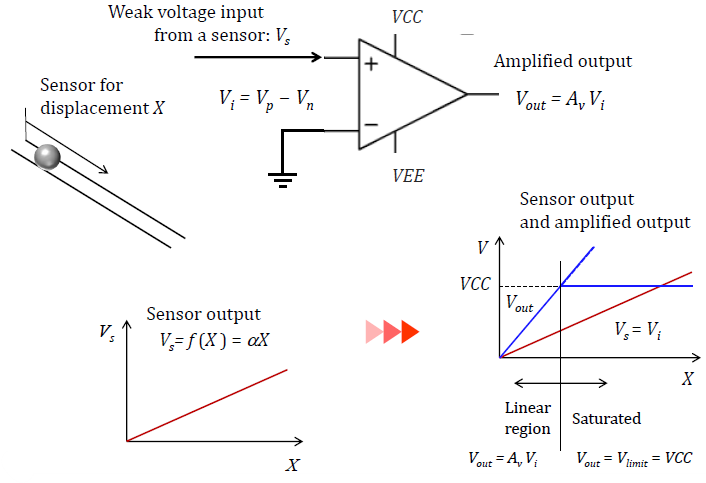
\includegraphics[width = 0.7\textwidth]{../img/diagram45.png}
\end{figure}
We can see that the signal is not infinitely amplified, as we are limited by the energy provided by our supply voltage. This is reflected in the graph above as the straight portion of the amplified line. This is called saturation. Due to $A_v$ being quite large, our linear region is normally tiny. This may be a problem if we want to measure the linear region.
\subsection{Negative feedback}
So op-amps seem to be a useful device but also seem to be a bit tricky. They are much more useful when used as part of a larger circuit. Negative feedback is achieved by feeding a fraction of the output signal back to the \textbf{inverting} terminal as shown. By definition, the closed-loop gain of such a device is:
\begin{equation}
  G = \frac{V_0}{V_i}
\end{equation}
\begin{figure}[H]
  \centering
  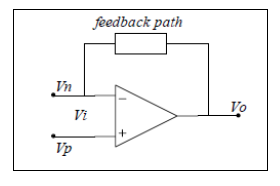
\includegraphics[width = 0.5\textwidth]{../img/diagram46.png}
\end{figure}
Negative feedback trades a reduction in gain with one that is smaller, stable and predictable, whilst giving the designer control over operational characteristics.
\subsection{Basic feedback amplifier configurations}
Only 2 resistors are required to construct a negative feedback amplifier. Note that output signal is always fed-back to the inverting input terminal.
\begin{figure}[H]
  \centering
  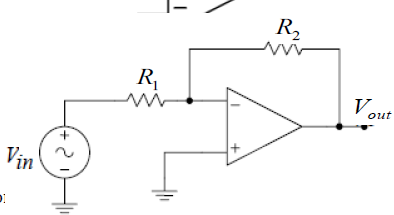
\includegraphics[width = 0.5\textwidth]{../img/diagram47.png}
  \caption{Inverting feedback amplifier arrangement.}
\end{figure}
\begin{figure}[H]
  \centering
  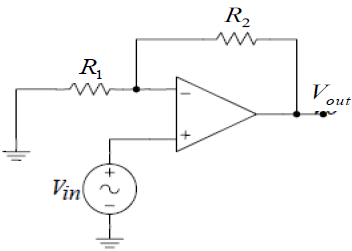
\includegraphics[width = 0.5\textwidth]{../img/diagram48.png}
  \caption{Non-inverting feedback amplifier arrangement.}
\end{figure}
We can see the difference between an inverting and non-inverting feedback amplifier is which input the source signal is connected to.
\subsection{Basic inverting feedback amplifier}
\begin{figure}[H]
  \centering
  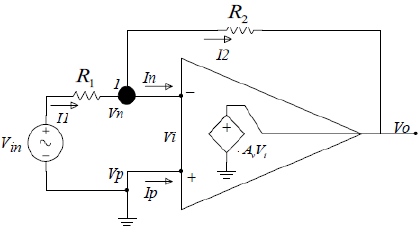
\includegraphics[width = 0.5\textwidth]{../img/diagram49.png}
\end{figure}
Let us derive its closed loop gain $G$. By definition:
\begin{gather}
  V_0 = A_v(V_p - V_n)\\
  V_p \rightarrow 0 \Longrightarrow V_n = - \frac{V_0}{A_v} \label{invertingfb1}
\end{gather}
Apply KCL to Node 1:
\begin{gather}
  \frac{V_{in}-V_n}{R_1} - I_n - \frac{V_n - V_0}{R_2} = 0 \Longrightarrow \frac{R_2}{R_1}V_{in} + v_n \left( 1 + \frac{R_2}{R_1} \right) = V_0 \label{invertingfb2}
\end{gather}
$I_n$ is 0 from our model assumptions.
Combining equations (\ref{invertingfb1}) and (\ref{invertingfb2}), we arrive at: 
\begin{gather}
  G \equiv \frac{V_0}{V_{in}} = -\frac{R_2}{R_1} \frac{1}{1 + \frac{1}{A_v}\left( 1 + \frac{R_2}{R_1}\right)}
\end{gather}
For an ideal op-amp, $A_v \rightarrow \infty$:
\begin{equation}
  G = \frac{V_0}{V_{in}} = - \frac{R_2}{R_1}
\end{equation}
\subsection{Basic non-inverting feedback amplifier}
\begin{figure}[H]
  \centering
  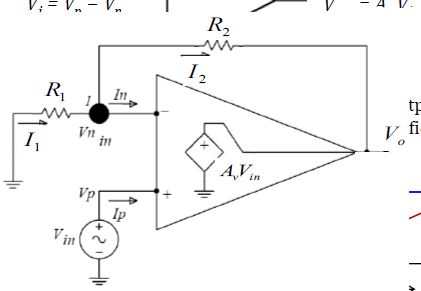
\includegraphics[width = 0.5\textwidth]{../img/diagram50.png}
\end{figure}
Derive its closed-loop gain $G$. By definition:
\begin{equation}
  V_0 = A_v (V_p - V_n) \label{noninvertingfb1}
\end{equation}
Apply KCL to node 1
\begin{gather}
  \frac{0 - V_n}{R_1} = \frac{V_n - V_0}{R_2} \rightarrow \frac{V_0}{R_2} = V_n \left(\frac{1}{R_1} + \frac{1}{R_2}\right) \label{noninvertingfb2}
\end{gather}
Combining equation (\ref{noninvertingfb1}) and (\ref{noninvertingfb2}), we arrive at:
\begin{equation}
  G \equiv \frac{V_0}{V_{in}} = \frac{1 + \frac{R_2}{R_1}}{1 + \frac{1}{A_v}\left(1 + \frac{R_2}{R_1}\right)}
\end{equation}
For an ideal amplifier, $A_v \rightarrow \infty$:
\begin{equation}
  G = 1 + \frac{R_2}{R_1}
\end{equation}
This is positive and always greater than 1.
\subsection{Summary}
\subsubsection*{Ideal feedback amplifier characteristics}
\begin{center}
  \begin{tabularx}{0.8\textwidth} { 
    | >{\centering\arraybackslash}X 
    | >{\centering\arraybackslash}X 
    | >{\centering\arraybackslash}X | }
    \hline
    & \textbf{Inverting amplifier} & \textbf{Non-inverting amplifier} \\
    \hline
    \hline
    $G = \frac{V_0}{V_{in}}$ & $-\frac{R_2}{R_1}$ & $1 + \frac{R_2}{R_1}$\\
    \hline
    $R_{in}$ & $R_1$ & $\infty$\\
    \hline
    $R_{out}$ & 0 & 0\\
    \hline
  \end{tabularx}
\end{center}
\subsection{Voltage amplification summary}
Operational amplifier:
\begin{itemize}
  \item The gain usually is too large (typically > 100,000) and not well defined. ($V_0$ cannot be larger than supply voltage)
  \item The gains for two op-amps of the same type can differ by a factor of two or more.
  \item The gain is not stable, can change with temperature, can change with changes of supply voltage.
\end{itemize}
To reduce these effects, we use negative feedback.
\begin{figure}[H]
  \centering
  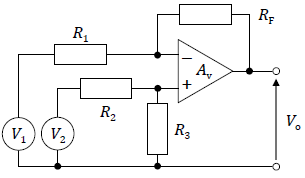
\includegraphics[width = 0.5\textwidth]{../img/diagram51.png}
  \caption{$V_1$ and $V_2$ could come from a Wheatstone bridge.}
\end{figure}
The output voltage $V_0$ is given as: 
\begin{gather}
  V_0 = \frac{R_F}{R_1}(V_2 - V_1)
\end{gather}
Only when $\frac{R_2}{R_3} = \frac{R_F}{F_1}$. This is independent of $A_v$ and the gain of this circuit, $G = \frac{R_F}{R_1}$ is well controllable.
\subsection{Difference amplifier}
Combining a non-inverting and inverting op-amp to take the difference between two inputs:
\begin{figure}[H]
  \centering
  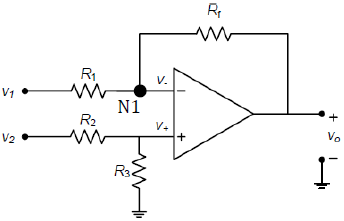
\includegraphics[width = 0.5\textwidth]{../img/diagram52.png}
\end{figure}
\begin{gather}
  \frac{V_0}{A_v} = V_+ - V_- \rightarrow 0 \textrm{ as } A_v \rightarrow \infty\\
  V_+ = \frac{R_3}{R_2 + R_3} \leftarrow \textrm{ voltage divider} \label{difamp1}
\end{gather}
KCL at node N1
\begin{gather}
  \frac{V_0 - V_-}{R_f} = \frac{V_- V_1}{R_1} \rightarrow \frac{V_0}{R_f} + \frac{V_1}{R_1} = \left(\frac{1}{R_f} + \frac{1}{R_1}\right)V_-\\
  \frac{V_0}{R_f} + \frac{V_1}{R_1} = \left(\frac{R_f + R_1}{R_f R_1}\right)\left(\frac{R_3}{R_2 + R_3}\right)V_2 \label{difamp2}
\end{gather}
Combining equation (\ref{difamp1}) and (\ref{difamp2}), we arrive at:
\begin{gather}
  V_0 = R_f \left(\frac{R_f + R_1}{R_f R_1}\right)\left(\frac{R_3}{R_2 + R_3}\right)V_2 - \frac{R_f}{R_1} V_1\\
  V_0 = \frac{1 + \frac{R_f}{R_1}}{1 + \frac{R_2}{R_3}}V_2 - \frac{R_f}{R_1}V_1
\end{gather}
If we can make sure that $\frac{R_f}{R_1} = \frac{R_3}{R_2}$ is satisfied, we can further reduce our equation to:
\begin{gather}
  V_0 = \frac{R_f}{R_i}(V_2 - V_1)
\end{gather}

\end{document}